\section{Evaluación experimental}

Las medidas salen de 160 corridas sobre 16 configuraciones, diez repeticiones
cada una, en un equipo con procesador Intel Core i7-1260P de 16 hilos, núcleo
Linux 6.18 bajo WSL2, GCC 13.3.0, glibc 2.39 y Python 3.12.3. Ninguna corrida
quedó descartada.

Antes de cada configuración se corre una repetición de calentamiento que se
descarta y queda declarada en el registro de la corrida. No es cosmética: la
primera corrida después de compilar llegó a medir la mitad que las siguientes
para el mismo trabajo, y promediarla habría metido el estado frío de la caché
dentro del resultado.

Las métricas de tráfico no las informa la aplicación: se derivan del registro
del coordinador. Los bytes incluyen los 32 de cabecera de cada trama, y la
página se cuenta una sola vez por transmisión. La desviación es la muestral.

\subsection{Localidad de lectura}

Un escritor publica una versión y un lector hace $M$ lecturas de la página
entera. Lo único que cambia es cuándo pide permiso: una sola adquisición para
las $M$ lecturas, o una por lectura. El trabajo local es idéntico en los dos
casos y está medido: las mismas $M$ verificaciones de 4096 bytes.

\begin{table*}[t]
\caption{Localidad de lectura con dos nodos y un lector.}
\label{tab:localidad}
\centering
\small
%% Generado por scripts/tablas_informe.py. No editar.
\begin{tabular}{@{}rlrrrrr@{}}
\toprule
lect. & permiso & tiempo (ms) & adq. & msjs. & bytes & págs. \\
\midrule
1 & una sola & $0,166 \pm 0,111$ & 1 & 22 & 13\,160 & 3 \\
1 & una por lectura & $0,139 \pm 0,026$ & 1 & 22 & 13\,160 & 3 \\
8 & una sola & $0,177 \pm 0,019$ & 1 & 22 & 13\,160 & 3 \\
8 & una por lectura & $1,157 \pm 0,172$ & 8 & 50 & 14\,168 & 3 \\
64 & una sola & $0,690 \pm 0,191$ & 1 & 22 & 13\,160 & 3 \\
64 & una por lectura & $8,056 \pm 0,679$ & 64 & 274 & 22\,232 & 3 \\
\bottomrule
\end{tabular}

\end{table*}

La última columna es el resultado: \textbf{tres páginas transferidas en los
seis casos}. Pedir permiso 64 veces en vez de una no mueve un solo byte de
datos extra en concepto de página; mueve mensajes. El tiempo pasa de 0,69 a
8,06~ms, 11,7 veces más, y los mensajes de 22 a 274.

La otra mitad del resultado es la fila que no cambia. Con una sola
adquisición, el costo en mensajes es 22 con 1, con 8 y con 64 lecturas: una
vez que el permiso está, leer es gratis en la red. La figura~\ref{fig:localidad}
muestra las dos cosas a la vez.

\begin{figure*}[t]
\centering
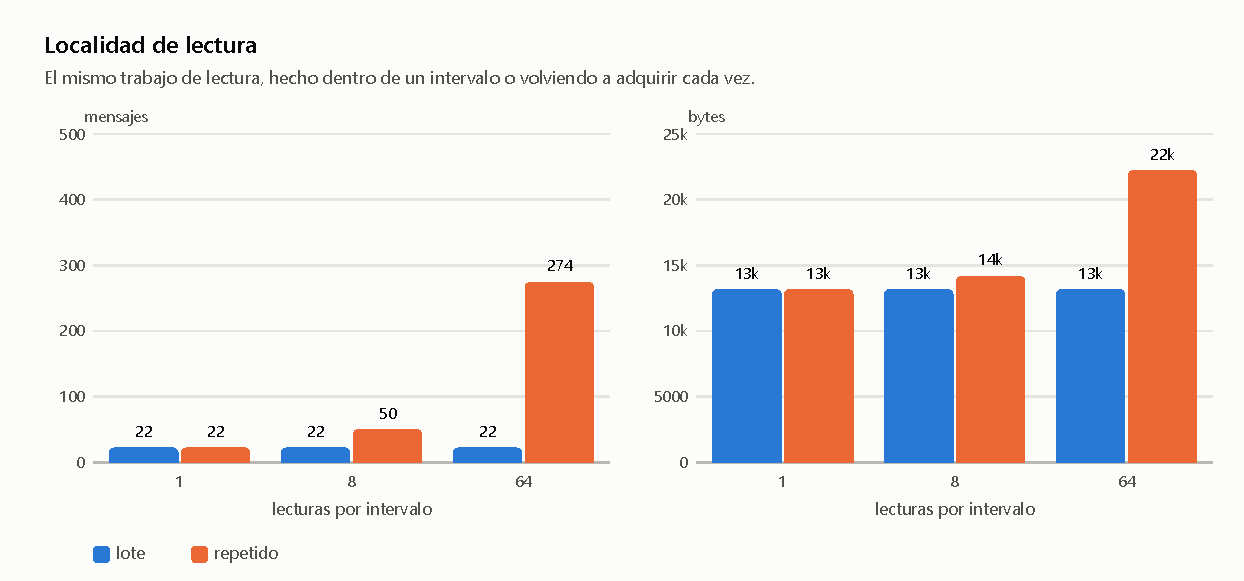
\includegraphics[width=0.86\textwidth]{figuras/fig1_localidad.pdf}
\caption{Mensajes y bytes según cuántas lecturas caben en una adquisición.}
\label{fig:localidad}
\end{figure*}

Los 13\,160 bytes de base no son del experimento: son el establecimiento de la
sesión, la publicación del escritor y las barreras. Por eso el crecimiento
relativo en bytes (1,7 veces) es mucho menor que el crecimiento en mensajes
(12,5 veces): lo que se agrega son tramas de 40 bytes, no páginas de 4096.

\subsection{Falso compartimiento}

Cada nodo incrementa \emph{su propio} contador 50 veces. Nadie lee el contador
de otro. Lo único que cambia entre los dos diseños es dónde viven los
contadores: todos en la página 0, u uno por página. El trabajo lógico es el
mismo y también está medido: 50 adquisiciones de escritura y 50 incrementos
por nodo en los dos diseños.

\begin{table*}[t]
\caption{Falso compartimiento con 50 rondas. El tiempo es el del nodo más
lento. Los bytes de coordinación son los de las barreras que ordenan las
rondas.}
\label{tab:fs}
\centering
\small
%% Generado por scripts/tablas_informe.py. No editar.
\begin{tabular}{@{}rlrrrrr@{}}
\toprule
$N$ & contadores & tiempo (ms) & inval. & b.\ coher. & págs. & b.\ coord. \\
\midrule
2 & misma página & $22,05 \pm 1,11$ & $96,0 \pm 2,1$ & 832\,640 & 198 & 8\,160 \\
2 & una por nodo & $14,05 \pm 1,09$ & 0 & 433\,280 & 102 & 8\,160 \\
4 & misma página & $42,87 \pm 3,23$ & $198,6 \pm 0,7$ & 1\,692\,736 & 403 & 16\,320 \\
4 & una por nodo & $17,86 \pm 0,75$ & 0 & 866\,560 & 204 & 16\,320 \\
\bottomrule
\end{tabular}

\end{table*}

Compartir la página cuesta 1,57 veces el tiempo con dos nodos y 2,40 con
cuatro, para un trabajo que la aplicación considera independiente. Las
invalidaciones pasan de cero a 96 y a 198,6 en promedio, los bytes de
coherencia casi se duplican y las páginas transferidas también.

\begin{figure*}[t]
\centering
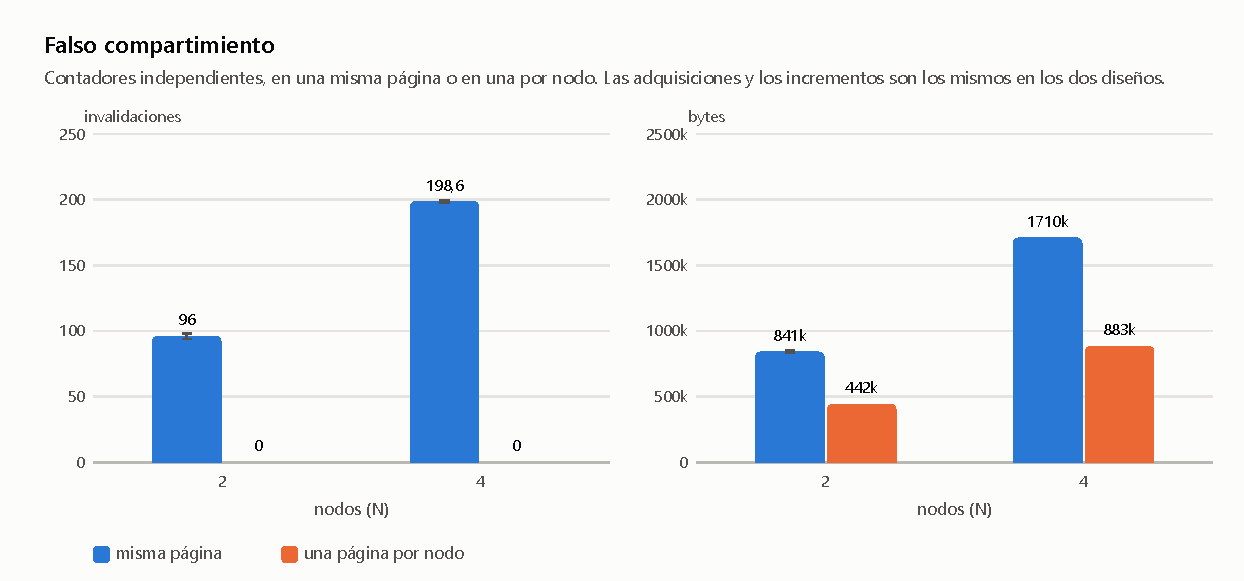
\includegraphics[width=0.86\textwidth]{figuras/fig2_false_sharing.pdf}
\caption{Invalidaciones y bytes según dónde viven contadores independientes.}
\label{fig:fs}
\end{figure*}

La columna que cierra el argumento es la última. Los bytes de coordinación son
\emph{idénticos} entre los dos diseños: 8\,160 con dos nodos y 16\,320 con
cuatro, en los dos casos. Las barreras que ordenan las rondas son las mismas,
así que no explican ninguna parte de la diferencia. Lo que cambia es
exclusivamente el tráfico de coherencia, y cambia porque la unidad de
coherencia es la página y no el dato.

\subsection{Costo de distribución}

La serie de Leibniz para $\pi$ con el mismo $T$ repartido entre $N$ nodos. Se
informan por separado el tiempo de la fase de cálculo y publicación, el total
de la sesión, y el de la serie secuencial de referencia que el nodo 0 calcula
para verificarse.

\begin{table*}[t]
\caption{Costo de distribución. La escala compara la fase de cálculo contra
la de un solo nodo con el mismo $T$.}
\label{tab:dist}
\centering
\small
%% Generado por scripts/tablas_informe.py. No editar.
\begin{tabular}{@{}rrrrrrr@{}}
\toprule
$T$ & $N$ & cálculo (ms) & total (ms) & secuencial (ms) & bytes & escala \\
\midrule
100\,003 & 1 & $0,47 \pm 0,06$ & $1,32 \pm 0,20$ & $0,22 \pm 0,03$ & 8\,776 & 1,00$\times$ \\
100\,003 & 2 & $0,61 \pm 0,23$ & $1,71 \pm 0,45$ & $0,22 \pm 0,05$ & 21\,568 & 0,77$\times$ \\
100\,003 & 4 & $0,89 \pm 0,14$ & $2,56 \pm 0,48$ & $0,20 \pm 0,00$ & 38\,960 & 0,53$\times$ \\
200\,000\,003 & 1 & $360,34 \pm 17,80$ & $712,01 \pm 33,35$ & $350,48 \pm 17,74$ & 8\,776 & 1,00$\times$ \\
200\,000\,003 & 2 & $209,56 \pm 19,40$ & $607,82 \pm 52,84$ & $396,88 \pm 37,34$ & 19\,520 & 1,72$\times$ \\
200\,000\,003 & 4 & $124,02 \pm 8,43$ & $567,71 \pm 17,30$ & $441,79 \pm 15,02$ & 37\,731 & 2,91$\times$ \\
\bottomrule
\end{tabular}

\end{table*}

Con $T$ grande la fase de cálculo escala 1,72 veces con dos nodos y 2,91 con
cuatro. El total baja mucho menos —de 712 a 568~ms— porque arrastra el
establecimiento de la sesión, las barreras y la serie de referencia, que no se
reparten entre nadie.

Con $T$ pequeño distribuir \emph{empeora} todo: el total sube de 1,32 a
2,56~ms al pasar de uno a cuatro nodos, y los bytes se multiplican por 4,4
mientras el cálculo tampoco baja. No hay nada que repartir, y lo único que se
mide es el costo de arrancar.

\begin{figure*}[t]
\centering
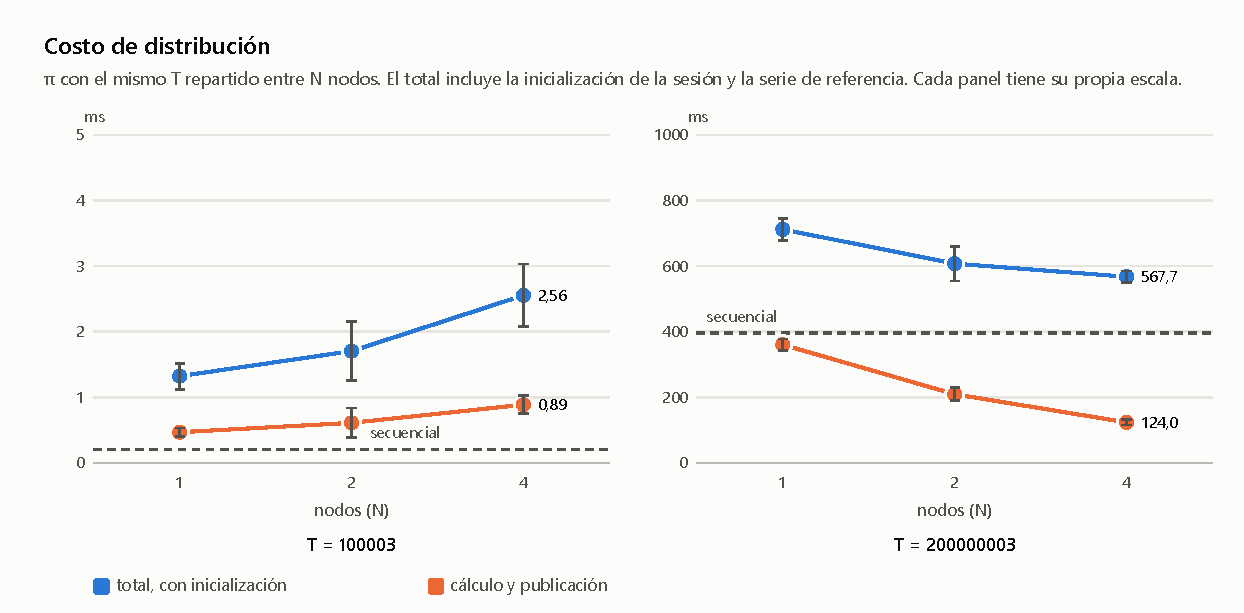
\includegraphics[width=0.86\textwidth]{figuras/fig3_distribucion.pdf}
\caption{Tiempo total y de la fase de cálculo contra la cantidad de nodos,
con la serie secuencial de referencia punteada. Cada panel tiene su escala.}
\label{fig:dist}
\end{figure*}

Hay una columna que no se puede leer como se leería en un banco de pruebas
limpio. El tiempo de la serie secuencial \emph{crece con $N$} —350~ms con un
nodo, 442 con cuatro— aunque el trabajo sea exactamente el mismo $T$. Esa
serie la calcula el nodo 0 mientras los demás procesos de la sesión están
vivos en la misma máquina, así que lo que mide de más es contención del
equipo, no del protocolo. La comparación que se sostiene es cálculo contra
cálculo, que es la que informa la columna de escala y la que dibuja la figura.
